\subsubsection{Testing during Development}
So far, we have looked at how unit tests and integration testing has been implemented, decomposed and combinated with CLS, making tests that conform to specific variations of the adventure game. Let us take a step back and look at the tests more specifically for a moment. Now that we have made it clear how the tests have been incorporated into our repository, let us discuss more about the testing itself, what we have accomplished with it and how it has helped us doing development. \\
In section '\nameref{BuildRep}' we discussed the implementation of grains with CLS and how we came to the conclusion that accepting dead code would make it easier to decompose the grains. One may then ask, how do we ensure that this dead code is in fact unreachable or atleast how can we be sure that it does not create any obvious flaw in our variations where the dead code resides. More generally one could ask, how do our test overall ensure that our variations actually work as intended. \\ 
Let us examine the question, how can we somewhat reliably state that dead code does not crash our code? We can take the example of the dead code in \autoref{PlayerTakeDamage} that is, the if statement with roarActive inside player's TakeDamage function, in the variations where we do not have roar. We can see in \autoref{IntegrationTakeDamage} how we tested the player's takeDamage.
\begin{figure}[]
    \centering
    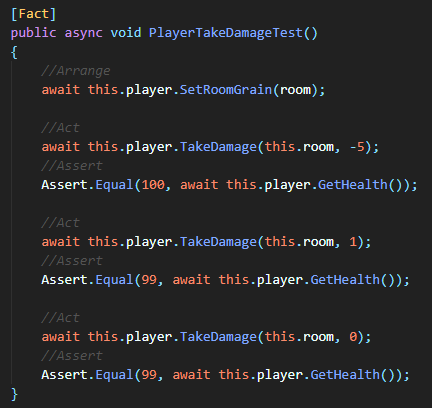
\includegraphics[width=0.6\linewidth]{Materials/TestingDiscussion/IntegrationTakeDamage}
    \caption{player's takeDamage in integration tests}
    \label{IntegrationTakeDamage}
\end{figure} 
As we only do black-box testing, we do not directly check the statements taken \todo{executed?} in TakeDamage while we test it. Instead, as we have mentioned in the section '\nameref{TestTheory}', we use equivalence classes and boundary testing to examine how our TakeDamage reacts to different input. This way we cannot say that the dead code will never cause problems, but we have tested the function with input from our equivalence classes such that we can deem it unlikely that this code will affect the program with the input that we can expect the TakeDamage to receive doing runtime. \\ \\
Other than testing as an end product and as a result of synthesis, we can also look at how it helped us during development of our grains and their functionality. As we tested alongside development of our grains, the tests gave us valuable insight into problems or bugs that appeared as we implemented functionality, but also ways to simplify our code, which helped as a way to make grains simpler for decomposition. As a small example, originally the player was to implement a heal function, such that upon entering a sunny room, the player's heal function would be called. However, this was the only use for this function. As testing exposed the fact that we could take negative damage that would result in healing the player instead, we scrapped the heal function and used TakeDamage instead. \\
Even though we have used these black-box testing methods, our testing is not complete. As we will discuss in the next section, making tests with Orleans and mockups did not go flawlessly and some of the functions proved difficult or downright impossible to test, at least during unit testing. we will look at some of the obstacles that came during testing and what we did to work around or solve this in the next section. 